% ---------------------------------------------------
%
% Proyecto de Final de Carrera: 
% Author: Álvaro Fontenla aluXXX@ull.edu.es
% Chapter: Preface
% File: Cap0_Preface.tex
%
% ----------------------------------------------------

\chapter*{Preface}
\addcontentsline{toc}{chapter}{Introduction} 

High Performance Computing (HPC) \cite{Assiroj:2018:High} is a practice that utilizes powerful processors in parallel to process big data and solve complex problems at incredibly high speeds.

All these processes analyze massive amounts of streaming data from IoT sensors, radar systems, and GPS in real time to make split-second decisions.
Higher performance in computer science is one of the key factors behind the evolution of hardware and software.
There exists a necessity for faster, more efficient calculus and data management.
The way we are able to fulfil this need has evolved with time.
For a significant number of decades, performance was increased by the upgrade in frequency of single-threaded CPUs, as seen on Figure \ref{fig:processor-trend}.
But there was a moment where an increase in frequency did not justify the also scaling power consumption.

\begin{figure}[H]
	\centering
	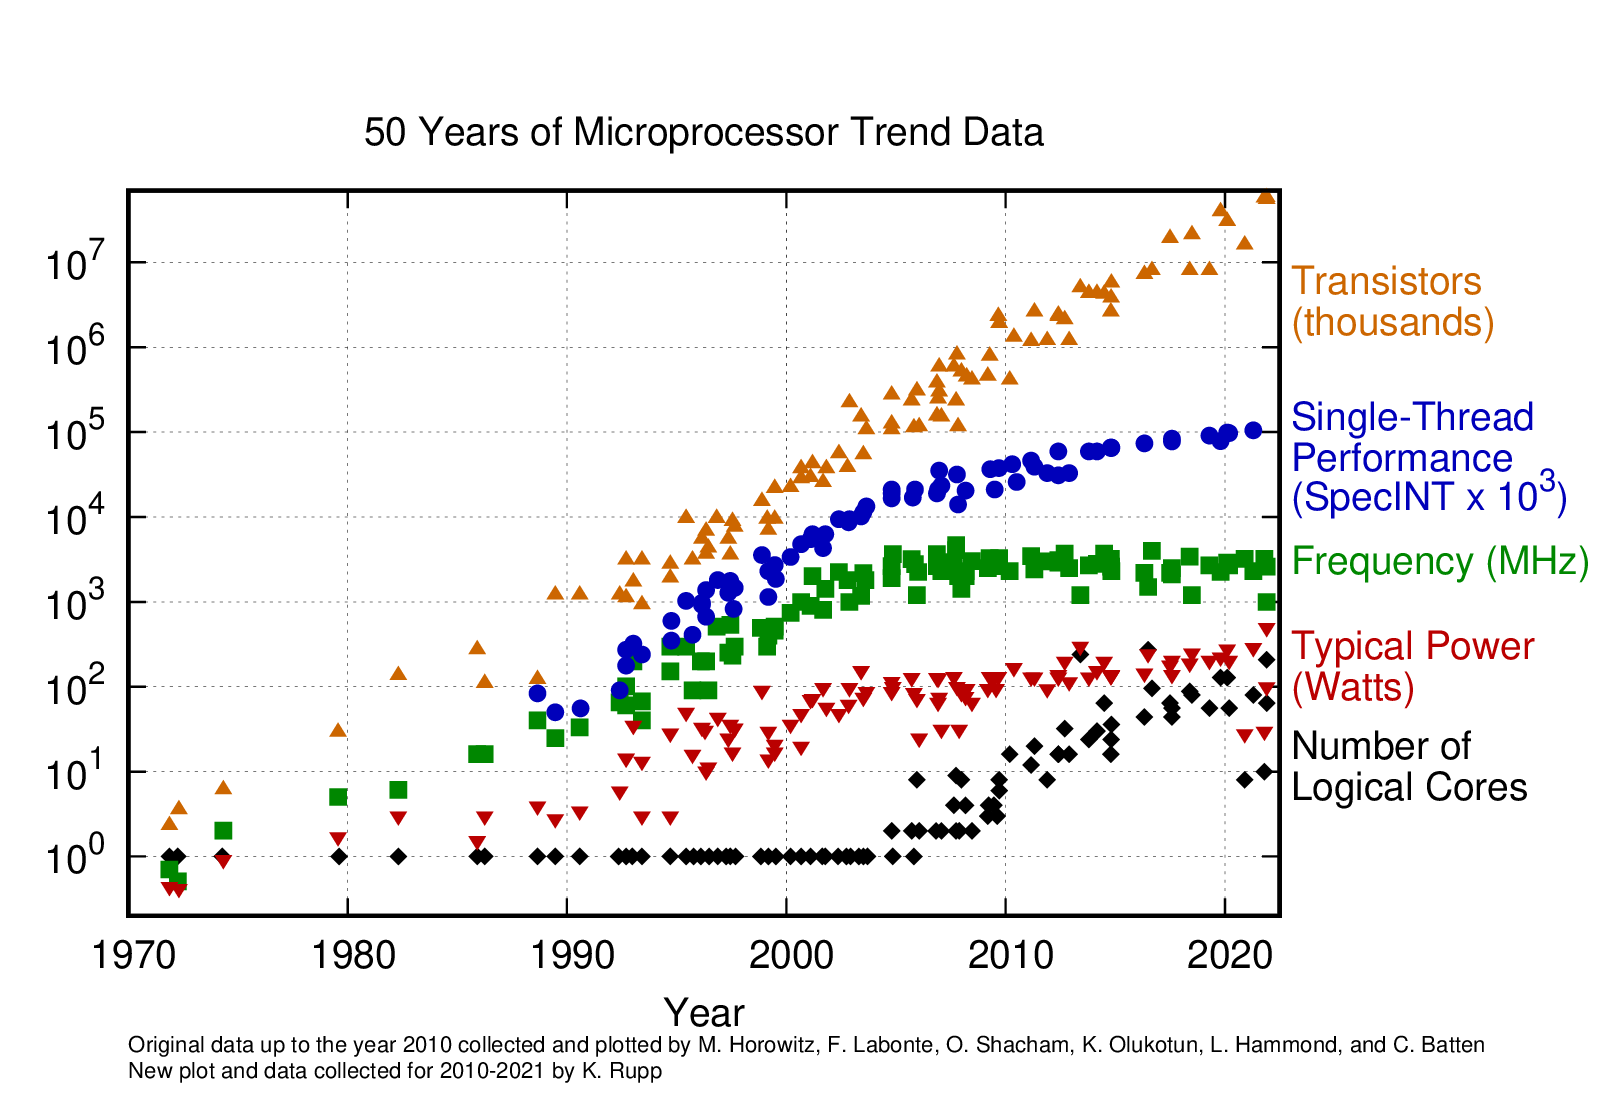
\includegraphics[width=\linewidth]{images/50-years-processor-trend.png}
	\caption{Trends of microprocessors.}
	\label{fig:processor-trend}
\end{figure}
